%% ============================================================
%% f2012_shandong_arts_q13_cube.tex
%% 2012 山东卷（文科）第 13 题 正方体 ABCD-A1B1C1D1，E 为 B1C 上一点
%% 来源 PDF：普通高考/2012/2012山东文.pdf 第 1 页（印面 761）第 2 栏
%% 坐标取自原页矢量层（bp），原点为图区左上角 (536.0,630.0)，y 向下；虚线照原页。
%% 第 628.05bp 处 31.5bp 的横线是题面填空横线，不属图稿，已排除。
%% ============================================================
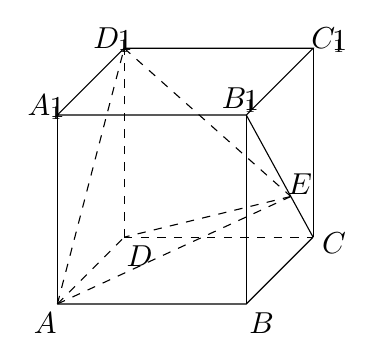
\begin{tikzpicture}[x=1bp,y=-1bp,
  every node/.style={inner sep=0,font=\fontsize{10.5pt}{12.6pt}\selectfont},
  line cap=butt, line join=miter]
  \draw[line width=0.398bp] (13.027,104.527) -- (81.035,104.527) -- (105.078,80.484);
  \draw[line width=0.398bp] (13.027,36.516) -- (81.035,36.516) -- (105.078,12.477) -- (37.07,12.477) -- (13.027,36.516);
  \draw[line width=0.398bp] (81.035,104.527) -- (81.035,36.516);
  \draw[line width=0.398bp] (105.078,80.484) -- (105.078,12.477);
  \draw[line width=0.398bp] (13.027,104.527) -- (13.027,36.516);
  \draw[line width=0.398bp] (81.035,36.516) -- (105.078,80.484);
  \draw[line width=0.398bp, dash pattern=on 2.989bp off 2.989bp] (13.027,104.527) -- (37.07,80.484);
  \draw[line width=0.398bp, dash pattern=on 2.989bp off 2.989bp] (37.066,80.484) -- (105.078,80.484);
  \draw[line width=0.398bp, dash pattern=on 2.989bp off 2.989bp] (37.066,80.484) -- (37.066,12.477);
  \draw[line width=0.398bp, dash pattern=on 2.989bp off 2.989bp] (37.066,12.477) -- (97.066,65.828);
  \draw[line width=0.398bp, dash pattern=on 2.989bp off 2.989bp] (97.066,65.828) -- (37.07,80.484);
  \draw[line width=0.398bp, dash pattern=on 2.989bp off 2.989bp] (13.027,104.527) -- (97.066,65.828);
  \draw[line width=0.398bp, dash pattern=on 2.989bp off 2.989bp] (13.027,104.527) -- (37.07,12.477);
  \node[anchor=base west] at (25.77,12.52) {$D_1$};
  \node[anchor=base west] at (34.47,13.41) {$1$};
  \node[anchor=base west] at (104.26,12.52) {$C_1$};
  \node[anchor=base west] at (111.77,13.41) {$1$};
  \node[anchor=base west] at (72.0,34.14) {$B_1$};
  \node[anchor=base west] at (79.97,35.03) {$1$};
  \node[anchor=base west] at (2.13,36.57) {$A_1$};
  \node[anchor=base west] at (10.0,37.46) {$1$};
  \node[anchor=base west] at (37.72,91.21) {$D$};
  \node[anchor=base west] at (95.79,65.17) {$E$};
  \node[anchor=base west] at (108.17,86.27) {$C$};
  \node[anchor=base west] at (4.37,115.26) {$A$};
  \node[anchor=base west] at (81.96,115.26) {$B$};
\end{tikzpicture}
